\newif\ifpreprint
 
%Preprint/reprint switch
\preprinttrue % Enable for single column preprint
%\preprintfalse % Enable for double column reprint
  
\ifpreprint
\documentclass[journal=jctcce,manuscript=article]{achemso}
\else
\documentclass[journal=jctcce,manuscript=article,layout=twocolumn]{achemso}
\fi

\usepackage[T1]{fontenc} % Use modern font encodings

\usepackage{amsmath}
\usepackage{newtxtext,newtxmath}

\usepackage{svg}
\usepackage{graphicx}
\usepackage{dcolumn}
\usepackage{braket}
\usepackage{multirow}
\usepackage{threeparttable}
\usepackage{xspace}
\usepackage{verbatim}
\usepackage[version=4]{mhchem} % Formula subscripts using \ce{}
\usepackage{comment}
\usepackage{color,soul}

\usepackage{mathtools}
\usepackage{xcolor}
\usepackage{xspace}
\usepackage{ifthen}

\usepackage{qcircuit}
\usepackage{booktabs,caption}

\newcommand*{\Eh}{$E_{\rm h}$\xspace}
\newcommand*{\Ecorr}{$E_{\rm{corr}}$\xspace}
%\newcommand*{\RCMnorm}{$\norm{\pmb{\lambda}_{2}}^{2}_{F}$\xspace}
%\newcommand*{\dRCMnorm}{$\norm{\pmb{\delta\lambda}_{2}}^{2}_{F}$\xspace}
\newcommand{\basis}[2]{\psi_{#1}^{({#2})}\xspace}
\newcommand{\familyabbr}[0]{QSD\xspace}
\newcommand{\familyname}[0]{Quantum Subspace Diagonalization\xspace}
\newcommand{\methodname}[0]{multireference selected quantum Krylov\xspace}
\newcommand{\methodabbr}[0]{MRSQK\xspace}
% the next two go together
\newcommand{\controlop}[1]{\mathrm{c}\mhyphen{#1}}

\mathchardef\mhyphen="2D

\providecommand{\norm}[1]{\lVert#1\rVert}

\usepackage[colorlinks = true,
            linkcolor = blue,
            urlcolor  = black,
            citecolor = blue,
            anchorcolor = black]{hyperref}

%\usepackage{lineno}
%\modulolinenumbers[5]
%\ifpreprint
%\setlength\linenumbersep{24pt}
%\else
%\setlength\linenumbersep{6pt}
%\fi
%\linenumbers

\definecolor{goodorange}{RGB}{225,125,0}
\definecolor{goodgreen}{RGB}{5,130,5}
\definecolor{goodred}{RGB}{220,50,25}
\definecolor{goodblue}{RGB}{30,144,255}
\definecolor{OliveGreen}{RGB}{5,100,5}


\usepackage{titlesec}
%\usepackage{footnote}
%
\let\titlefont\undefined
\usepackage[fontsize=11pt]{scrextend}
\captionsetup{font={sf,footnotesize}}
%
\titleformat{\section}
{\normalfont\sffamily\bfseries\color{OliveGreen}}
{\thesection.}{0.25em}{\uppercase}

\titleformat{\subsection}[runin]
{\normalfont\sffamily\bfseries}
{\thesubsection}{0.25em}{}[.\;\;]

\titleformat{\suppinfo}
{\normalfont\sffamily\bfseries}
{\thesubsection}{0.25em}{}


\titlespacing*{\section}{0pt}{0.5\baselineskip}{0.01\baselineskip}
\titlespacing*{\subsection}{0pt}{0.125\baselineskip}{0.01\baselineskip}

\renewcommand{\refname}{\normalfont\sffamily\bfseries\color{OliveGreen}{\normalsize  REFERENCES}} 



\author{Renke Huang}
\email{renke.huang@emory.edu}
\affiliation{Department of Chemistry and Cherry Emerson Center for Scientific Computation, Emory University, Atlanta, GA, 30322}

\setlength{\bibsep}{0pt plus 0.3ex}

% bibliography print title or not
%\setkeys{acs}{usetitle=true}


\let\oldmaketitle\maketitle
\let\maketitle\relax

\title{Ordering of Trotterization and Resource Estimation for Multireference Quantum Krylov Algorithm }

% \date{\today}

\begin{document}

%\oldmaketitle

%\begin{abstract}

%\end{abstract}

\section{Introduction}

Simulating fermions whose interactions display strong correlation effects on classical computers is plagued by the computational difficulties from the exponential growth of many-body Hilbert space dimension.\cite{Laughlin:2000br} 
This problem motivated the original idea of quantum computing.\cite{Feynman:1982gn,manin1980computable} 
The past decade has witnessed the milestone achieved in the hardware development of the quantum computer,\cite{Arute:2019fg} so it has become crucial to realize useful applications to demonstrate the potential it promises. Current noisy intermediate-scale quantum (NISQ) devices,\cite{Preskill:2018gt} characterized by 50 to several hundred qubits and low gate fidelity, limit the depth and width of quantum circuits that can be executed with sufficient confidence, which puts many constraints on the design of algorithms for quantum simulation.

Quantum computers have a prominent advantage for simulating quantum dynamics, the unitary time evolution of a highly-entangled state.\cite{Kassal:2008bf}
The quantum algorithm combining unitary evolution and phase estimation, termed QPE, was the first to manifest the exponential speedup in solving the eigenvalue problem of a local hamiltonian,\cite{Abrams:1997ha,Abrams:1999ur} and adapted for fermionic simulations.\cite{Ortiz:2001jn} 
Then QPE was applied to small molecules for calculating the ground-state energy,\cite{AspuruGuzik:dj} and later the complete spectrum on photonic hardware.\cite{Lanyon:2010jf}
However, for medium to large systems of chemical interest, such as FeMoco, the transition metal center in a nitrogenase enzyme, an estimate of circuit depth and coherence time needed for QPE is far beyond the reach of NISQ devices.\cite{Reiher:2017cv}
Promising alternatives tailored for the existing or near-term noisy hardware are hybrid quantum-classical algorithms. Two major schemes of this type are the variational quantum eigensolver (VQE)\cite{Peruzzo:2014kc,Yung:2014iv,McClean:2015bs} and the quantum approximate optimization algorithm (QAOA),\cite{Farhi:2014wl} both of which are variational. It has been shown that variational methods are more error/noise resilient than QPE.\cite{McClean:2017ct,Cao:2019jn}

The VQE algorithm leverages the quantum computer only for the classically intractable task, namely, preparing an entangled quantum state by a parametrized circuit termed the ansatz, and obtaining the energy expectation from statistics of repetitive measurements of the state.\cite{McClean:2015bs}
Then, a classical optimizer minimizes the energy and updates parameters iteratively. In this way, the VQE trades a polynomial overhead of measurements and classical optimization for a much shorter coherence time and a reduction of the circuit depth.\cite{McArdle:2019we}
The most important wavefunction ansatz in the VQE scheme is the unitary coupled cluster truncated at single and double excitations (UCCSD),\cite{McClean:2015bs, OMalley:2016dc, Barkoutsos:2018hm, Romero:2019hk} which is inspired by efforts in improving classical coupled cluster theory.\cite{bartlett1989alternative, kutzelnigg1991error, Szalay:1995vu, Taube:2006bi, Cooper:2010ck, Evangelista:2011eh, Harsha:2018dv}
Several variants of UCCSD ansatz have been explored, including $k$-UpCCGSD approach which utilizes generalized singles and doubles,\cite{Lee:2018cy} qubit UCC constructed directly from entangler gates\cite{Ryabinkin:2018jw,Ryabinkin:2019vh} with qubit mean-field reference,\cite{Ryabinkin:2018tv} Bogoliubov UCC using fermionic Gaussian state reference,\cite{DallaireDemers:2019iw} compact UCC with gradient-selected unitaries\cite{Grimsley:2019ed} and its two-qubit-gate-efficient variant\cite{Tang:2019ug}.
Other alternatives, primarily, hardware-efficient ansatzes that only use the set of gates easily implementable on NISQ devices\cite{Kandala:2017gh, M:2019hw, Rattew:2019wv} also gain attention because of much shallower circuits.
The VQE scheme has also been extended to compute excited-state properties,\cite{McClean:2017ct, Higgott:2018fca, Colless:2018hp, Parrish:2019bw, Nakanishi:2019wo, Jouzdani:2019tp, GreeneDiniz:2019tg, Tilly:2020tj} or combined with QPE to reduce the measurement cost.\cite{Wang:2019ha, Santagati:2018ih}
While VQE experiments have been realized on most existing hardware architectures,\cite{Peruzzo:2014kc,Yung:2014iv,OMalley:2016dc,Hempel:2018to,Colless:2018hp,Santagati:2018ih,Shen:2017cc,M:2019hw} multiple challenges nonetheless remain in practice $-$ the difficulty of high-dimensional classical optimization of the energy,\cite{McClean:2018kf} a large number of measurements required for converging the expectation value to high precision\cite{Barkoutsos:2019wq} and intrinsic accuracy limit from the inexact ansatz.\cite{Evangelista:2019kz} Therefore, it is crucial to improve the VQE further or to develop other hybrid algorithms.

The idea of representing the Hamiltonian in a non-orthogonal subspace,\cite{ostlund1982modern} which has various practices in classical computational chemistry,\cite{Lowdin:1950tq,King:1967ev,Noodleman:1981iz,Voter:1981eu,Malmqvist:1986jh,Koch:1993tf,thom2009hartree,sundstrom2014non} has also been adopted in a class of quantum-classical algorithms referred to as \familyname (QSD).\cite{McClean:2017ct,Colless:2018hp,Motta:2019bu, Parrish:2019tc,Huggins:2019vv,Ollitrault:2019tn,Takeshita:2020dh}
The initial proposal of QSD, named quantum subspace expansion (QSE), aimed at extending the VQE scheme to compute excited states and mitigate errors.\cite{McClean:2017ct} 
In this work, the Hamiltonian is expanded in the configuration interactions singles (CIS) subspace $\hat{a}_{i}^{\dagger} \hat{a}_{j}\ket{|\Psi}$, and overlap matrix elements are three- and four-electron reduced density matrices measured in VQE experiments by operator averaging.\cite{Takeshita:2020dh} Then solving the generalized eigenvalue problem yields both the ground and excited states. Nevertheless, the CIS basis only expands a relatively small, restricted Hilbert space. Diagonalization of the possible noisy Hamiltonian matrices in this space might lead to systematic biases.\cite{Blunt:2018ee}
Huggins \textit{et al.} developed another VQE-based QSD method, termed the non-orthogonal VQE (NOVQE) approach,\cite{Huggins:2019vv} which uses separate VQE experiments to generate and optimize a set of non-orthogonal $k$-UpCCGSD type states\cite{Lee:2018cy} and diagonalizes the Hamiltonian in this basis. One motivation of this work is to mitigate the difficulty of optimization in the context of VQE.

While many efforts in the QSD is to extend or augment the VQE scheme, the general QSD framework is likely to go beyond, specifically in terms of the great flexibility in the way to form the subspace. 
Motta \textit{et al.} proposed the Quantum Lanczos (QLanczos) algorithm\cite{Motta:2019bu} which fills a Krylov subspace with basis vectors in powers of $e^{-2\Delta \tau H}$ such that $\mathcal{K}: \{\ket{\Phi}, e^{-2 \Delta \tau H}\ket{\Phi}, e^{-4  \Delta \tau H}\ket{\Phi},…  \}$. These basis vectors are obtained using the QITE algorithm,\cite{Motta:2019bu} which maps the Trotterized\cite{Trotter:1959wh} imaginary-time propagator to a unitary operator scaled by the norm of the evolved state vector after a single Trotter time step. The matrix elements in the QLanczos are computed based on the expectations values of those mapped unitaries, which are available after direct measurements. Note that the QLanczos algorithm requires no classical optimization, and its convergence is guaranteed by properties of the imaginary-time evolution, free of fixed ansatz errors in its variational variant.\cite{McArdle:2019ek} These advantages show that the QSD scheme provides viable solutions to circumvent problems that hinder the VQE methods. 

Inspired by the QLanczos algorithm, we proposed a multireference selected quantum Krylov (MRSQK) method\cite{stair2019multireference} based on real-time dynamics, and also provided the circuit to evaluate matrix elements efficiently by indirect measurements (the Hadamard test),\cite{aharonov2009polynomial} which is distinct from the expectation value measuring in the situation of both the QSE\cite{McClean:2017ct} and the Qlanczos.\cite{Motta:2019bu}
QSD methods that generate the non-orthogonal basis from a single state are likely to suffer from numerical instabilities due to the linear dependency of basis states.\cite{Motta:2019bu,Huggins:2019vv} Thus, we initialized the QSD procedure with a set of orthogonal references.
When completing this work, we noticed a recent preprint paper by Parrish and McMahon\cite{Parrish:2019tc} which shares part of the ideas employed in our work. 
They theorized a quantum filter diagonalization approach (QFD) in which the variational basis is generated by propagating several reference states approximately in real-time, which is motivated by classical filter diagonalization\cite{Neuhauser:1994jp,Neuhauser:1990dp,wall1995extraction, mandelshtam1997low} and time-grid-propagation based quantum algorithms.\cite{Somma:2002jo,Somma:2019th,OBrien:2019cw,Kyriienko:2020gg} 
The QFD method is applied to simulate the spectrum of an 8-qubit \textit{ab initio} exciton Hamiltonian, where they started with the zero configuration $\ket{00...}$ and all singly-excited configurations \{$\ket{10...}$, $\ket{010...}$,...\}, and propagated these references to form a time-grid subspace.\cite{Parrish:2019tc}.
While we utilized the same strategy to produce basis states from a single reference, our method has the novelty that real-time dynamics on the mean-field reference and measurements are also used to automatically select important configurations with large amplitudes out and add them to the set of references. The selection procedure preserves symmetries, such as the particle number, the total spin, the spatial symmetry, making it fit for the fermionic Hamiltonian, which is generally more complicated than the exciton model.


%%%%%%%%%%%%%%%%%
%\section{Theory}
\section{Results and Discussion}

\subsection{Basis in \methodabbr}

The \methodname method combined with real-time dynamics generates a $d(s+1)$-dimensional non-orthogonal Krylov space $\mathcal{K}$ in the form 
\begin{equation}
\begin{split}
\label{krylov}
\mathcal{K} : \{ & \ket{\Phi_{0}}, e^{-i \Delta t \hat{H}} \ket{\Phi_{0}}, e^{-i 2 \Delta t \hat{H}} \ket{\Phi_{0}}, ... , e^{-i s\Delta t \hat{H}} \ket{\Phi_{0}}, \\
& \ket{\Phi_{1}}, e^{-i \Delta t \hat{H}} \ket{\Phi_{1}}, e^{-i 2 \Delta t \hat{H}} \ket{\Phi_{1}}, ... ,e^{-i s\Delta t \hat{H}} \ket{\Phi_{1}}, \\
& ... \\
& \ket{\Phi_{d-1}}, e^{-i \Delta t \hat{H}} \ket{\Phi_{d-1}}, e^{-i 2 \Delta t \hat{H}} \ket{\Phi_{d-1}}, ... ,e^{-i s\Delta t \hat{H}} \ket{\Phi_{d-1}}  \}  
\end{split}
\end{equation}
This is done in two successive procedures, including the \textit{reference selection} and the \textit{reference propagation}.

The \textit{reference selection} utilizes the real-time evolution of a single Slater determinant $\ket{\Phi_0}$ (usually the Hartree-Fock reference) to determine other $(d-1)$ references.
It starts with propagating $\ket{\Phi_0}$ at fixed intervals in real-time, which forms a trial time-grid basis $\{\ket{\Phi_0}, e^{-i\Delta t \hat{H}} \ket{\Phi_0}, e^{-i2\Delta t \hat{H}} \ket{\Phi_0}...\}$ with $(s^{\prime}+1)$ dimension.
The ground state of the Hamiltonian in this trial basis is written as
\begin{equation}
\ket{\widetilde{\Psi}_{0}} = \sum_{k=0}^{s^{\prime}} C_{0 k} \, e^{-i k \Delta t \hat{H}} \ket{\Phi_{0}}
= \sum_{k=0}^{s^{\prime}} C_{0 k}  \ket{k}
\end{equation}
We use Jordan-Wigner transform\cite{jordan1993paulische} to map the fermionic Fock space to the Hilbert space of qubits.\cite{whitfield2011simulation} In this mapping, a Slater determinant in the Fock space is represented by a qubit computational basis state that has the same binary representation. Note that the algorithm is agnostic to the encoding method, but in order to give a chemically-intuitive picture, that determinants (fermionic basis states) and computational basis states are the same in the Jordan-Wigner encoding, we can conveniently view these two bases equivalently in the following explanation.
Each time-grid basis vector $\ket{k}$ can be written as a linear combination of $n$-qubit computational basis states (Slater determinants) $\ket{k} = \sum_{\mu} C_{k \mu} \ket{\mu}$. Then, the trial ground state vector can be decomposed in the computational basis
\begin{equation}
\label{trial_gs}
\ket{\widetilde{\Psi}_{0}} = \sum_{k=0}^{s^{\prime}} \sum_{\mu=0}^{2^{n}-1}  C_{0 k} \, C_{k \mu} \ket{\mu} 
\end{equation}
Based on Eq. \ref{trial_gs}, the probability of measuring the determinant $\ket{\mu}$ in the trial ground state $\ket{\widetilde{\Psi}_{0}}$ is given by $P_{\mu}=|\sum_{k=0}^{s^{\prime}} C_{0 k} C_{k \mu}|^{2}$.
$\ket{\widetilde{\Psi}_{0}}$ can also be written in a compact way as the Hadamard product\cite{horn2012matrix} (element-wise multiplication) of three vectors $\ket{\widetilde{\Psi}_{0}} = \sum_{k} \mathbf{C_{0}}  \circ  \mathbf{C_{k }}   \circ \,  \vec{\mu}$,
where $\vec{\mu}$ comprises all the n-qubit computational basis states $\vec{\mu} = (\ket{0}, \ket{1}, ... ,\ket{2^{n}-1})$.

The coefficient vector $\mathbf{C_{0}} = (C_{00}, C_{01}, ... , C_{0s^{\prime}} )$ is obtained by solving the generalized eigenvalue problem,
\begin{equation}
\label{ge}
\mathbf{HC} = \mathbf{SCE}
\end{equation}
with matrix elements given by 
$S_{\alpha \beta} = \bra{\Phi_0} e^{i \alpha \Delta t \hat{H}} e^{-i \beta \Delta t \hat{H}} \ket{\Phi_0} $,
$\ H_{\alpha \beta} = \bra{\Phi_0} e^{i \alpha \Delta t \hat{H}}  \hat{H}   e^{-i \beta \Delta t \hat{H}}  \ket{\Phi_0}$,
where $\alpha, \beta \in [0,1,...,s^{\prime}]$. $\mathbf{C_{0}}$ is the eigenvector corresponding to the lowest eigenvalue.

$\mathbf{C_{k }}$ is the state vector of the quantum state $\ket{k} = e^{-i k \Delta t \hat{H}} \ket{\Phi_0} = \sum_{\mu} C_{k \mu} \ket{\mu}$, which can be simulated classically (e.g. statevector simulator in the \texttt{Qiskit-Aer}\cite{Qiskit} package). However, in real experiments, the state vector cannot be directly read out from the quantum computer. 
Available quantities from projective measurements on a quantum state are 
$\mathbf{bin}(\mu)$, the binary representation of the determinant $\ket{\mu}$ to which the state collapes after measuring $\ket{k}$ in the computational basis, 
and $|C_{k \mu}|^2$, the probability of getting $\ket{\mu}$.\cite{rieffel2011quantum}
While the exact value of any $C_{k \mu}$, which is complex in general, can not be determined, we can nonetheless use $|C_{k \mu}|^2$ to upper bound the probability of sampling the determinant $\ket{\mu}$ in the trial ground state $\ket{\widetilde{\Psi}_{0}}$:
\begin{equation}
P_{\mu} =  | \sum_{k=0}^{s^{\prime}}  C_{0 k} C_{k \mu}  |^2   
\leqslant  \sum_{k} |C_{0 k} |^{2}  |C_{k \mu}|^{2} 
\end{equation}
which follows from the Cauchy-Schwarz inequality.
The upper bound expression is adopted in practice for the probability estimation.
To make it more explicitly, we prepare time-grid basis states $\{\ket{k}\}$ separately on multiple quantum computers. Each quantum computer outputs a probability distribution $\{|C_{\mu} |^{2}\}_{\mu}$ of determinants. 
The overall probability of a single $\ket{\mu}$ is computed as the weighted sum over the probability of $\ket{\mu}$ in each time-grid basis state. 
Note that we only use the value of $P_{\mu}$ to select important states, so a qualitatively correct measurement statistics of the time-evolved state is sufficient for our need, which means not many measurement repetitions are required. 

Through finite measurements, we form a coarse aggregate of important determinants and sort them in descending order according to the overall probability. 
Next, the set is refined, such that only determinants with the same particle number as $\ket{\Phi_0}$ are kept. 
Then, we enforce the total spin symmetry by leaving the closed-shell configurations alone as one state, grouping open-shell configurations with the same spin occupation pattern to zero out the total spin, summing their weights, and normalizing the obtained multi-configurational states.
Lastly, we select $d-1$ largest-weighted states, together with $\ket{\Phi_0}$, to form our reference set $\{ \ket{\Phi_{I}} \}_{I=0}^{d-1}$.
The \textit{reference propagation} then fills the Krylov space with states sampled at fixed intervals when evolving each reference.

Diagonalizing the Hamiltonian in the entire $d(s+1)$-dimensional space $\mathcal{K}$ requires solving Eq. \ref{ge} again, with more general matrix representations of the overlap $\mathbf{S}$ and the Hamiltonian $\mathbf{H}$ given by
\begin{align}
\label{overlap_eq}
S_{I(s+1)+\alpha,\; J(s+1)+\beta} &= \bra{\Phi_I} e^{i \alpha \Delta t \hat{H}} e^{-i \beta \Delta t \hat{H}} \ket{\Phi_J}, \\
\label{hamiltonian_eq}
H_{I(s+1)+\alpha,\; J(s+1)+\beta} &= \bra{\Phi_I} e^{i \alpha \Delta t \hat{H}} \hat{H} e^{-i \beta \Delta t \hat{H}} \ket{\Phi_J}
\end{align}
where $\alpha, \beta \in [0,1,...,s]$, $I, J \in [0,1,...,d-1]$, indices are consistent with the basis ordering in Eq. \ref{krylov}. 

%%%%%%%%%%%%%%%%
\subsection{State Preparation} 

Given a qubit Hamiltonian after the Jordan-Wigner\cite{jordan1993paulische} or the Bravyi-Kitaev encoding,\cite{Bravyi2002, Seeley:2012em} in general, not all Pauli terms (tensor products of Pauli operators) in the Hamiltonian commute.
\begin{equation}
\hat{H}=E_{0}+\sum_{l}^{N} h_{l} \bigotimes_{k=1}^{n} \sigma_{k}^{\{I, X, Y, Z\}}
\end{equation}
One may realize the time evolution operator $e^{-i t \hat{H}}$ on a quantum computer following the widely-used first order Lie-Trotter-Suzuki product approximation\cite{Trotter:1959wh, Suzuki:1991fz, hatano2005finding} or higher-order product formulae\cite{Suzuki:1976cf, Berry:2007iw}. 
Other more sophisticated methods include truncated Taylor series expansions,\cite{Berry:2015ir, Babbush:2016bx}
linear combinations of unitaries (LCU),\cite{Childs:2012cg}
Chebyshev polynomial approximations,\cite{Subramanian:2019ex} 
or the recently proposed qubitization\cite{Low:2019kr, Berry:2019bb} in conjunction with quantum signal processing\cite{Low:2017kn} methods.
In our case, the first-order Lie-Trotter-Suzuki product with $m$ Trotter steps (numbers) is employed
\begin{equation}
e^{-i t \hat{H}}=\left(\prod_{l}^N e^{-i \frac{t h_{l}}{m} \bigotimes_{k} \sigma_{k}}\right)^{m} 
+ O\left(\frac{(t h_{l})^{2}} {m}\right)
\end{equation}
The error in approximating $e^{-i t \hat{H}}$ using product formula is determined by both the number of Trotter steps and the Trotter order. 
In the first-order Trotter-Suzuki formula, the number of Trotter steps required for a simulation error of $\epsilon$ scales as $m = O((t h_{l})^{2} / \epsilon)$, so $m$ should be large to suppress approximation errors. 

It has been observed that in practice, the first order Trotter-Suzuki product gives errors in the ground state energy scaling as $1/m^2$,\cite{Hastings:2015uj} same as that of second-order Trotter-Suzuki approximation. Therefore, considering both the error scaling and the state preparation cost, the first-order formula that has much shorter circuits is favorable.

We argue that the \methodabbr method is likely to achieve better error scaling than the Trotter error, because it has the variational optimization of the state when solving the generalized eigenvalue problem in a subspace, while variational methods are shown to be resilient to errors to some extent.\cite{McClean:2015bs, OMalley:2016dc}

%%%%%%%%%%%%%%%%%%%%%%%%%%%%%%%%%%
\subsection{Quantum Circuits for Measuring Matrix Elements} 

 In order to compute matrix elements on quantum devices, we use a modified Hadamard test\cite{Somma:2003jz} (shown in Fig.~\ref{circ_hadamard}) to measure observables indirectly with the help of one ancilla qubit. To explain it more detailedly, we reformulate Eq. \ref{overlap_eq} and Eq. \ref{hamiltonian_eq}, denoting collective indices $\gamma = (I, \alpha)$, $\chi = (J, \beta)$, and the $l$-th tensor product in the qubit Hamiltonian $\hat{P}_l =  \bigotimes_{k=1}^n \sigma_{k}^{\{I,X,Y,Z\}}$
\begin{align}
\label{s_reform}
S_{\gamma \chi} 
& = \braket{\bar{0} | \hat{U}_I^\dagger \; (\prod_{l} e^{i \frac{\alpha \Delta t h_{l}}{m} \hat{P}_l  } )^{m}  \vdots    
( \prod_{l} e^{- i \frac{\beta \Delta t h_{l}}{m}  \hat{P}_l  } )^{m}   \;    \hat{U}_J  |  \bar{0}  }  
= \braket{\bar{0} | \hat{U}_I^{\dagger}   \hat{U}_\alpha^{\dagger}   \hat{U}_\beta    \hat{U}_J  |  \bar{0}  }
= \braket{\bar{0} | \hat{U}_\gamma^{\dagger}  \hat{U}_\chi  |  \bar{0}  }  \\
\label{h_reform}
H_{\gamma \chi} 
& = \braket{\bar{0} | \hat{U}_I^\dagger \; (\prod_{l} e^{i \frac{\alpha \Delta t h_{l}}{m} \hat{P}_l  } )^{m}  \hat{H}
( \prod_{l} e^{- i \frac{\beta \Delta t h_{l}}{m}  \hat{P}_l  } )^{m}   \;    \hat{U}_J  |  \bar{0}  } 
= E_0 \braket{\bar{0} | \hat{U}_\gamma^{\dagger}  \hat{U}_\chi  |  \bar{0}  }  +\sum_l^N   h_l  \braket{\bar{0} | \hat{U}_\gamma^{\dagger} \,  \hat{P}_l   \,  \hat{U}_\chi  |  \bar{0}  }
\end{align}
$\hat{U}_I$, $\hat{U}_J$ are unitary oracles that output reference states. For a single determinant (one computational basis state), $\hat{U}_{\{I,J\}}$ comprises one layer of X gates. Protocols for constructing multi-determinant states are proposed\cite{Sugisaki:2016kx, Tubman:2018wz, Sugisaki:2019fz} with linear scaling in the number of qubits. 
In the most general case when matrix elements are between basis states that evolve from different references $\ket{\Phi_I}$, $\ket{\Phi_J}$, we need to implement the controlled reference oracles $\controlop{\hat{U}_{\{I,J\}}}$, which have two-qubit gates at the same scaling as single-qubit gates in $\hat{U}_{\{I,J\}}$.
While for matrix elements between states from the same reference $\ket{\Phi_I}$, we simplify Eq. \ref{s_reform}, \ref{h_reform} as $S_{\gamma \chi}=\braket{\Phi_I |  \hat{U}_\alpha^{\dagger}  \hat{U}_\beta  |  \Phi_I  }$,
$H_{\gamma \chi}=E_0 \braket{\Phi_I |  \hat{U}_\alpha^{\dagger}  \hat{U}_\beta  |  \Phi_I  }  + \sum_l h_l \braket{\Phi_I |  \hat{U}_\alpha^{\dagger}  \hat{U}_\beta  |  \Phi_I  }$,
where only the series of exponentials of $\hat{P}_I$ are included in the controlled unitaries, with $\hat{U}_{\{I=J\}}$ gulped in the main register state preparation.

\begin{figure}[bh!]
\[ \Qcircuit @C=1em @R=.7em {
& \lstick{\ket{\bar{0}}}        &\qw          & \qw          & \gate{\hat{U}_\gamma}  &   \qw          & \gate{\hat{U}_\chi}      & \qw     \\
& \lstick{\ket{0} }      &\gate{H}   & \gate{X}             & \ctrl{-1}  \qwx                   & \gate{X}        & \ctrl{-1}  \qwx           &   \rstick{\braket{X+iY}}   \qw  \\  
% \measure{\mbox{$2\sigma_{+}$}} 
} \]
\caption{Hadamard test circuit to estimate expectation values of unitary operators with a general form of $\braket{\bar{0} | \hat{U}_\gamma^\dagger  \hat{U}_\chi | \bar{0}} $. Measuring the $X$, $Y$ operators on the ancillary qubit $\ket{0}$, one can obtain the mean value of $X+iY = 2 \ket{0}\bra{1}$, which equals to $\braket{X+iY} = \braket{\bar{0} | \hat{U}_\gamma^\dagger  \hat{U}_\chi  | \bar{0}} $ }
\label{circ_hadamard}
\end{figure}

The method to exponentiate tensor products of Pauli gates is described in Ref.~\citenum{Seeley:2012em, Hastings:2015uj}. The exponential of one $\hat{P}_l=\bigotimes_{k} \sigma_{k}$ is given by
\begin{equation}
e^{-i t_{l} \otimes_{k} \sigma_{k}} = \left(    \bigotimes_{k=1}^n H_k^\dagger  \right) 
\left( \prod_{i=1}^{n-1}  \mathrm{CNOT}_{i,i+1}  \right)
e^{-i t_{l}  \sigma_{n}^Z} 
\left( \prod_{i=n-1}^{1}  \mathrm{CNOT}_{i,i+1}  \right)
\left(    \bigotimes_{k=1}^n H_k  \right) 
\end{equation}
where $H_k$ gates perform transformations between the eigenbasis of $\sigma^X$ or $\sigma^Y$ and $\sigma^Z$, i.e. $H_k^\dagger  \sigma^{\{X, Y\}}  H_k = \sigma^Z$, $t_l = \alpha \Delta  t  h_l / m$
and $e^{-i t_{l}  \sigma_{n}^Z}  = R_z(2t_l)$ represents the $Z$ rotation gate on the qubit with the largest index.

For applying $e^{-i t_{l} \otimes_{k} \sigma_{k}}$ on the main register controlled by the ancillary qubit, we only need to replace the $R_z(2t_l)$ with a controlled $R_z(2t_l)$ on the last qubit, as illustrated in Fig.~\ref{cic_c-exp}. In this way, $l$ terms in a single Trotter step are executed sequentially. For larger Trotter number $m$, we just run $m$ replicas of $l$-terms in series.

\begin{figure}[h!]
\[
\Qcircuit @C=.45em @R=.6em {
 &    & \gate{H_{1}}       & \ctrl{1} & \qw       & \cds{5.5}{\cdots} & \qw        & \qw                           & \qw     & \cds{5.5}{\cdots}   & \qw      & \ctrl{1}   & \gate{H_{1}^\dagger}        & \qw\\
&    & \gate{H_2}       & \targ    & \ctrl{1}  &\qw                       & \qw       & \qw                            & \qw     & \qw                        & \ctrl{1}  & \targ     & \gate{H_2^\dagger}        & \qw \\
 &    & \gate{H_3}       & \qw      & \targ     & \qw                      & \qw       & \qw                           & \qw      & \qw                        & \targ     & \qw      & \gate{H_3^\dagger}         & \qw \\
 %&    &                              &             &            &                             &             &                                  &             &                              &             &             &                               & \\
 &    & \gate{H_{n-1}} & \qw      & \qw       & \qw                      & \ctrl{1}  & \qw                           & \ctrl{1}   & \qw                       & \qw      & \qw       & \gate{H_{n-1}^\dagger} & \qw \\
 &    & \gate{H_n}       & \qw      & \qw      & \qw                       & \targ     & \gate{R_z(2t_l)}  & \targ      & \qw                       & \qw      & \qw       & \gate{H_n^\dagger}      & \qw \\
&  \lstick{\ket{0}_{\mathrm{a}}}     & \qw                       & \qw      & \qw      & \qw                       & \qw.       & \ctrl{-1} \qwx                   & \qw        & \qw                       & \qw      & \qw       & \qw                         & \qw   %\\
\inputgroup{2}{3} {.8em} {\ket{\Phi}}    %{.8em}{.8em}
}\]
\caption{Circuit for applying one $\mathrm{controlled-}e^{-i t_{l} \otimes_{k} \sigma_{k}}$ operator.}
\label{cic_c-exp}
\end{figure}


To give readers an idea of how to construct such circuits in practice, we demonstrate an example circuit to compute several matrix elements for a two-qubit molecular \ce{H2} Hamiltonian\cite{OMalley:2016dc} using the spin symmetry-enforced Bravyi-Kitaev transformation,\cite{Moll_2016, Bravyi:2017wb} at the bond length of 0.75~\AA{}. Coefficients $h_l$ are computed in STO-3G basis given in Table I of the supplementary information of Ref.~\citenum{Colless:2018hp}. 
\begin{equation}
\hat{H}_q = -0.349833 - 0.388748\sigma_0^Z  + 0.181771\sigma_0^X \sigma_1^X - 0.388748 \sigma_1^Z + 0.011177\sigma_0^Z \sigma_1^Z
\end{equation}
Four determinants are mapped to computational basis states explicitly as 
$\ket{00} = a_{0 \alpha}^{\dagger} a_{0 \beta}^{\dagger}  \ket{\mathrm{vac}}$, 
$\ket{01} = a_{0 \alpha}^{\dagger} a_{1 \beta}^{\dagger}  \ket{\mathrm{vac}}$, 
$\ket{10} = a_{1 \alpha}^{\dagger} a_{0 \beta}^{\dagger}  \ket{\mathrm{vac}}$, 
$\ket{11} = a_{1 \alpha}^{\dagger} a_{1 \beta}^{\dagger}  \ket{\mathrm{vac}}$, 
The Hartree-Fock state for this Hamiltonian is $\ket{\Phi_0} = \ket{00}$.
A normalized spin adapted Krylov basis reference state is given by $\ket{\Phi_1}= (\ket{01} + \ket{10} ) / \sqrt{2}$.
The \methodabbr parameters used in evaluating one matrix element are set, with the time grid $\Delta t = 0.1$, the number of Trotter step(s) $m=1$.  
We take two off-diagonal matrix elements as examples, which are overlaps between Krylov basis state $\ket{\Phi_1}$ and $e^{-i \Delta t \hat{H}_q }  \ket{\Phi_1}$, $e^{-i \Delta t \hat{H}_q }  \ket{\Phi_0}$ and $\ket{\Phi_1}$.
Hadamard test circuits with one-step Trotter-Suzuki approximation to compute $\braket{\Phi_1  | e^{-i \Delta t \hat{H}_q}  |  \Phi_1}$ and $\braket{\Phi_0  | e^{i \Delta t \hat{H}_q}  |  \Phi_1}$
by estimating $\braket{X+iY}_\mathrm{anc}$ are shown in Fig.~\ref{h2_cir}, where the ancilla qubit is measured to obtain $\braket{Y}$.
Substituting the final $U2(\pi/2, -\pi/2)$ gates with Hadamard gates in two circuits will give $\braket{X}$. 

\begin{figure}[h!]
  \centering
  %\includesvg{phi01_cir4y.svg}
  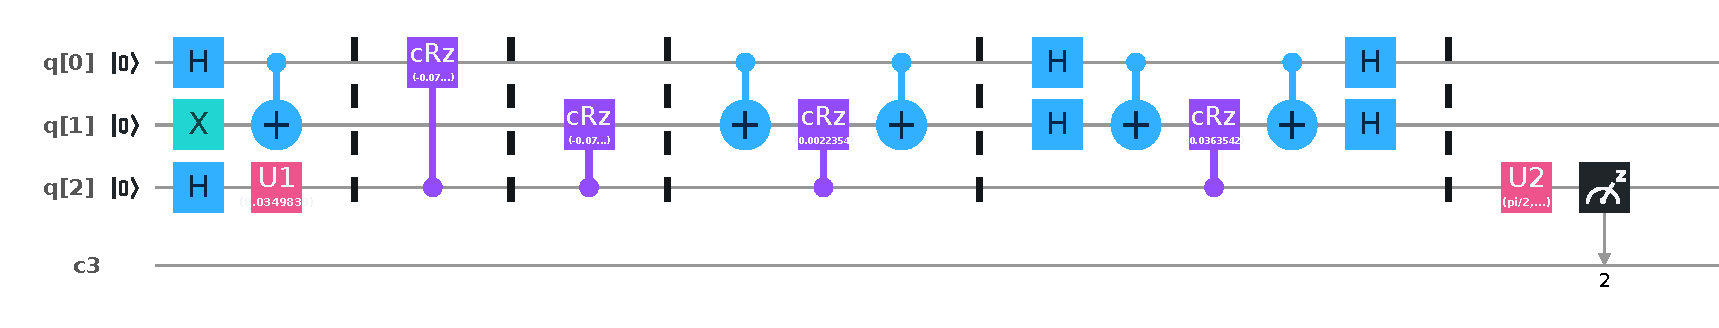
\includegraphics[width=6.5in]{figs/phi1_cir4y.pdf}
  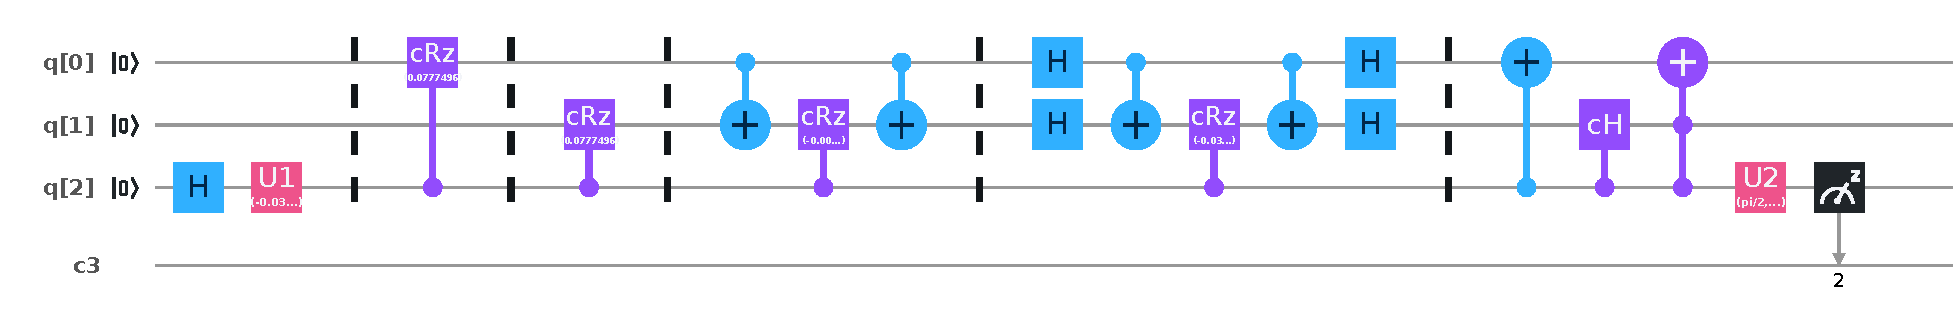
\includegraphics[width=6.5in]{figs/phi0+e1_cir_y.pdf}
  \caption{The circuit to compute $\braket{\Phi_1  | e^{-i \Delta t \hat{H}_q}  |  \Phi_1}$ (top) and $\braket{\Phi_0  | e^{i \Delta t \hat{H}_q}  |  \Phi_1}$ (bottom) implemented using \texttt{Qiskit}\cite{Qiskit}. \textbf{q[0]}, \textbf{q[1] }encode basis states for the Hamiltonian, while \textbf{q[2]} is the ancillary qubit, with \textbf{c3} the classical bit to store the output from measuring \textbf{q[2]}. $U2(\pi/2, -\pi/2)$ gate before the measurement is the $H_k$ gate rotating the state of ancillary qubit into the $\sigma^Y$ basis.  }
\label{h2_cir}
\end{figure}

%%%%%%%%%%%%%%%%
\subsection{Cost Estimation}

\begin{table*}[!ht]
\centering
\renewcommand{\arraystretch}{1.1}
\caption{
Resource estimates for \methodabbr calculations with $m=1$ Trotter step approximation on several hydrogen systems in STO-6G basis at the bond length R=1.5 \AA.
Jordan-Wigner transformation is used to encode the Hamiltonian for all cases in the table. }
\footnotesize
\begin{tabular*}{\columnwidth}{@{\extracolsep{\fill}}*{1}{r}*{8}{r}@{}}    %9: means 9 columns for right ones
%\begin{tabular*}{\columnwidth}{| c | c | c | c | c | c | c |}    % \stretch{0.4}
\hline
\toprule
\,  &  \ce{H2}  &   \ce{H4} (linear)  &  \ce{H_4} (ring)   &  \ce{H6} (linear)   &   \ce{H6} (ring)  &   \ce{H8} (linear)      \\
\midrule
 Num. of qubits   &  4   &   8   &   8   &   12   &  12   &   16  \\
 Num. of Pauli terms   &  14    &   184    & 92       &  918     &  702     &  2912   \\ [3pt]
 Num. of $H$/$R_{zy}$ ($H_k$) gates       &  16   &   480     &	 224    &   2832	&   2240     &   9664    \\
 Num. of 1-qubit gate layers	                  &	  8     &   296     &	 112    &  1680	&   1248     &   5552         \\[3pt]
 Num. of CNOT gates                                &  36    &  1328   &  520      &  9972     &  7476      & 41600    \\
 Num. of $\controlop{R_z}$ gates           &  14    &  184     &    92       &  918       &   702       &  2912   \\  [3pt]
 Num. of total layers                                   &  58    &  1808  &    724     &  12570   &   9426    &  50064 \\
\bottomrule
\hline
\end{tabular*}
\label{cost_table}
\end{table*}

The quantum resource cost in the \methodabbr method is dominated by the number of two-qubit gates in the controlled Hamiltonian exponentials, especially the CNOT gates. 
Here we present a rough estimate of the gate counts in measuring matrix elements at the minimal Trotter step ($m=1$), summarized in Table~\ref{cost_table}. 

The concept of circuit depth can be interpreted as layers in a circuit.\cite{rieffel2011quantum}
The layer counting follows the rule that the set of gates that can be executed concurrently in parallel contributes one layer of the circuit.
It is clear that in the $\controlop{e^{-i H t}}$ circuit we are interested in, the number of layers of single-qubit basis change gates $H_k$ are roughly half of the total 1-qubit gate counts, while each two-qubit gate adds one layer to the circuit, because they need to run sequentially in the time order.
Denoting the number of terms (tensor products of single-qubit Pauli gates) in the Hamiltonian $N$, the weight of each term $w_l$ (the number of  non-identity ($\sigma^I$) Pauli gates in one term), the Trotter number $m$, a boolean quantity $\delta_l^Z$ that sets to 1 if at least one Pauli gate in the tensor product is $\sigma^X$ or $\sigma^Y$, else sets to 0, 
we give estimates of gate counts by
\begin{align}
\label{cost_formula}
\bar{N}_\mathrm{1-q}  & =  m \sum_l^N  2 w_l   \\
\bar{N}_\mathrm{CNOT} & =  m \sum_l^N  2 (w_l - 1)  \\
\bar{N}_\mathrm{R_z}  & = N m  \\
\bar{N}_\mathrm{layer}  & = m \sum_l^N  (2 w_l + 2 \delta_l^Z - 1) 
\end{align}

Note that all the numbers in the table serve as upper bounds for the implementation in practice, because we analyze the case when the number of qubits is equal to the number of spin orbitals with the active space spanning the whole molecular orbital space. 
Also, a direct application of the Jordan-Wigner transformation retains some redundant degrees of freedom in the qubit Hamiltonian and states.
Other more advanced encoding techniques enable the quantum simulation with fewer qubits. 
For example, Temme \textit{et al.}\cite{Bravyi:2017wb}  described a transform to remove qubits in the presence of $\mathbb{Z}_{2}$ symmetries.
On the other hand, these circuits can be further compressed and compiled. By carefully choosing the term order, it is likely to cancel some basis change gates $H_k$ and CNOT gates between two adjacent term exponentials, because all quantum gates are unitary and reversible. In this way, the number of gates will be much fewer than the ones reported in the table.

%%%%%%%%%%%%%%%%%%%%%%%%%%%%%
\subsection{Numerical Studies: Trotterization and Pauli Term Ordering}

The \methodabbr algorithm was implemented using the open-source quantum computer simulator \texttt{QForte}.\cite{Evangelista2019QForte}
All integrals required in the qubit Hamiltonian are computed by \texttt{Psi4}\cite{Parrish:2017hg} and transformed via the Jordan-Wigner encoding in \texttt{OpenFermion}.\cite{McClean:2017tj}

We present numerical results on the linear \ce{H6} and \ce{BeH2} to benchmark the performance of the \methodabbr method.
The linear hydrogen chains are known to have strong electron correlations of diverse nature as the bond length changes.\cite{Sinitskiy2010StrongCorrelation,  stella2011strong, Motta2017TowardsThe, Motta:2019ts} 
The symmetric stretching of the Be-H bond is also a typical model system for the benchmark study on multi-reference methods.  
 
Errors in the \methodabbr computations largely come from the Trotter-Suzuki approximation of the real-time dynamics. 
We consider two factors that affect the approximation error, the number of Trotter steps $m$, and the ordering of Pauli term exponentials in the circuit. 
It is interesting to examine how effectively the ordering of terms helps to mitigate the Trotter error when the number of Trotter steps is small. Because if a likely optimal ordering is used, we can achieve the same accuracy by a smaller $m$ compared to that in other orderings.

%%%%%%%%%%% Ground States Table%%%%%%%%%%%%
\begin{table*}[!ht]
\centering
\renewcommand{\arraystretch}{1.1}
\caption{Ground-state energies (in \Eh) of \textbf{linear \ce{H6}} at a bond distance of 1.5~\AA{}. \methodabbr results are given for $N = d (s+1)$ Krylov basis states using three steps ($s = 3$) and $\Delta t = 0.5$ a.u.
$m$ indicates the Trotter number.
Subscripts denote different ordering type of Pauli terms in the qubit Hamiltonian after the Trotterization. 
\textbf{OF}: OpenFermion's default QubitOperator ordering; 
\textbf{JW}: terms are sorted in the descending order based on the magnitude of coefficients after \textit{Jordan-Wigner} transform (Pauli term with largest magnitude goes first);
\textbf{sq}: terms are sorted in the descending order based on the magnitudes of amplitudes of fermion operators in the \textit{second quantized} form of the Hamiltonian (the group of terms from the fermion operator with the largest amplitude go first).
\textbf{rand}: Pauli terms are shuffled \textit{randomly} after Jordan-Wigner transform.
}
\footnotesize
\begin{tabular*}{\columnwidth}{@{\extracolsep{\fill}}*{1}{r}*{8}{r}@{}}    %9: means 9 columns for right ones
%\begin{tabular*}{\columnwidth}{| c | c | c | c | c | c | c |}    % \stretch{0.4}
 \hline
 \toprule
     $N$    &    $E^{(m=1)}_{\rm{OF}}$    &    $E^{(m=1)}_{\rm{JW}}$    &    $E^{(m=1)}_{\rm{sq}}$    &    $E^{(m=1)}_{\rm{rand}}$     &     $E^{(m=2)}_{\rm{OF}}$    &    $E^{(m=2)}_{\rm{JW}}$     &   $E^{(m=2)}_{\rm{sq}}$    &     $E^{(m=2)}_{\rm{rand}}$       \\
\midrule
    4    &    $-$2.982186    &    $-$2.988497   &   $-$2.988691   &   $-$2.982186   &    $-$2.998858   &    $-$3.001573    &  $-$3.002303    &   $-$2.998858  \\
    8    &    $-$3.001195	  &    $-$3.010441   &   $-$3.010010   &   $-$3.001195   &    $-$3.010035   &    $-$3.014902     &  $-$3.015058   &   $-$3.010035  \\	
  12    &    $-$3.008661	  &    $-$3.010831   &   $-$3.010532   &   $-$3.008661   &    $-$3.013425   &    $-$3.015151   &   $-$3.015306    &   $-$3.013425  \\
  16    &    $-$3.010543	  &    $-$3.011343   &   $-$3.011179   &   $-$3.010543   &    $-$3.014253   &    $-$3.015388   &   $-$3.015527    &   $-$ 3.014253  \\
  20    &    $-$3.011663    &    $-$3.016956   &   $-$3.017073   &    $-$3.011663  &    $-$3.015311   &    $-$3.018432   &    $-$3.018505   &    $-$3.015311  \\
\hline
\toprule
  $N$    &     $E^{(m=4)}_{\rm{OF}}$    &   $E^{(m=4)}_{\rm{JW}}$    &   $E^{(m=4)}_{\rm{sq}}$   &   $E^{(m=4)}_{\rm{rand}}$   &     $E^{(m=8)}_{\rm{OF}}$    &   $E^{(m=8)}_{\rm{JW}}$    &   $E^{(m=8)}_{\rm{sq}}$   &   $E^{(m=8)}_{\rm{rand}}$   \\
  \midrule
  4      &   $-$3.009948   &    $-$3.009826    &    $-$3.010353   &   $-$3.009948      &   $-$3.014138    &   $-$3.013367    &   $-$3.013629    &   $-$3.014138  \\
  8      &   $-$3.015872   &    $-$3.017784    &    $-$3.017966   &   $-$3.015872      &   $-$3.018341    &   $-$3.018880    &   $-$3.018970    &   $-$3.018341  \\
  12    &   $-$3.016940   &    $-$3.017891    &   $-$3.018062    &   $-$3.016940      &   $-$3.018808    &   $-$3.018956    &   $-$3.019039    &   $-$3.018808  \\
  16    &   $-$3.017173   &    $-$3.017980    &   $-$3.018152    &   $-$3.017173      &   $-$3.018888    &   $-$3.019012    &   $-$3.019105    &   $-$3.018888  \\ 
  20    &    $-$3.017614  &    $-$3.019231    &   $-$3.019280    &   $-$3.017614     &    $-$3.019054   &    $-$3.019669   &    $-$3.019710     &    $-$3.019054   \\[3pt]
~~~FCI       &  $-$3.020198    &   \textit{c.a. thres.}      &    $-$3.018604   \\% chemical accuracy
\bottomrule
\hline
\end{tabular*}
\label{h6_gse_table}
\end{table*}

%%%%%%%%%%% 1st-Excited States Table%%%%%%%%%%%%
\begin{table*}[!ht]
\centering
\renewcommand{\arraystretch}{1.1}
\caption{First excited-state energies (in \Eh) of \textbf{linear \ce{H6}} at a bond distance of 1.5~\AA{}. \methodabbr results are given for $N = d (s+1)$ Krylov basis states using three steps ($s = 3$) and $\Delta t = 0.5$ a.u.
Notations are consistent with those in Table~\ref{h6_gse_table}.}
\footnotesize
\begin{tabular*}{\columnwidth}{@{\extracolsep{\fill}}*{1}{r}*{9}{r}@{}}    
 \toprule
     $N$     &    $E^{(m=2)}_{\rm{OF}}$    &    $E^{(m=2)}_{\rm{JW}}$     &   $E^{(m=2)}_{\rm{sq}}$    &     $E^{(m=2)}_{\rm{rand}}$    &   $E^{(m=4)}_{\rm{OF}}$    &   $E^{(m=4)}_{\rm{JW}}$    &   $E^{(m=4)}_{\rm{sq}}$    &    $E^{(m=4)}_{\rm{rand}}$  \\
     \midrule
  8      &   $-$2.813678   &    $-$2.822952   &    $-$2.819339   &   $-$2.813678     &   $-$2.854913    &   $-$2.851219   &   $-$2.850036   &   $-$2.854913  \\
 16       &   $-$2.822238   &    $-$2.847035   &    $-$2.842780  &   $-$2.822238     &   $-$2.859053    &   $-$2.867098   &   $-$2.865905   &   $-$2.859053  \\
  24      &   $-$2.831772   &    $-$2.854135  &    $-$2.849167   &   $-$2.831772     &   $-$2.866840   &   $-$2.874047   &   $-$2.872074   &   $-$2.866840  \\
  32      &   $-$2.844701   &    $-$2.860495   &    $-$2.856910   &   $-$2.844701     &   $-$2.870509    &   $-$2.878594   &   $-$2.877274   &   $-$2.870509  \\
 \hline
 \toprule
  $N$    &     $E^{(m=8)}_{\rm{OF}}$    &   $E^{(m=8)}_{\rm{JW}}$    &   $E^{(m=8)}_{\rm{sq}}$   &   $E^{(m=8)}_{\rm{rand}}$   &     $E^{(m=100)}_{\rm{OF}}$    &   $E^{(m=100)}_{\rm{JW}}$    &   $E^{(m=100)}_{\rm{sq}}$   &   $E^{(m=100)}_{\rm{rand}}$   \\
  \midrule
  8        &   $-$2.865878   &    $-$2.862217   &    $-$2.861961   &   $-$2.865878     &   $-$2.868958    &   $-$2.868574   &   $-$2.868583   &   $-$2.868958  \\
  16      &   $-$2.870392  &    $-$2.873199   &    $-$2.873127   &   $-$2.870392     &   $-$2.874589    &   $-$2.876091   &   $-$2.876461   &   $-$2.874589  \\
  24      &   $-$2.877971   &    $-$2.879774   &    $-$2.879015   &   $-$2.877971            &   $-$2.882155    &   $-$2.882154   &   $-$2.882124   &   $-$2.882155  \\
  32      &   $-$2.880205   &    $-$2.883214   &    $-$2.882670   &   $-$2.880205           &   $-$2.884504   &   $-$2.884840    &   $-$2.884817   &   $-$2.884504  \\[3pt] 
~~~FCI       &  $-$2.889922         \\  % -2.888328 
\bottomrule
\hline
\end{tabular*}
\label{h6_1stese_table}
\end{table*}
%%%%%%%%%%% END 1st-Excited States Table%%%%%%%%%%%%

Table~\ref{h6_gse_table} shows the ground-state energies from \methodabbr computations with the Trotter number $m$ of 1, 2, 4, 8, and four ordering strategies for linear \ce{H6} at a bond length of 1.5~\AA.
We observe that chemical accuracy (error less than 1 kcal mol$^{-1}$ = 1.594 m\Eh) can be reached fastest if \textbf{sq} ordering is used. 
For example, when $m=4$, \methodabbr using \textbf{sq} ordering gives an error of 0.917~m\Eh with 20 Krylov basis states, while \textbf{JW} ordering gives 0.967~m\Eh, and both the \textbf{OF} and \textbf{rand} ordering have a much larger error of 2.584~m\Eh.
To see the effect of ordering clearly, we compare the energy errors with respect to FCI for different orderings in several Trotter number $m$ as a function of the number of Krylov basis states $N$, displayed in Fig.~\ref{h6_error-N}.
It is clear to find two patterns of asymptotic convergences. For this specific \ce{H6} geometry, \textbf{sq} and \textbf{JW} ordering always converge faster than \textbf{OF} and \textbf{rand} ordering. 
While there is a small difference between \textbf{sq} energies and \textbf{JW}  energies, numbers of \textbf{OF} and \textbf{rand}  are exactly the same to at least 6 decimals. 
Other random orderings are also tested (not shown), but all of them give the same results as \textbf{OF} and \textbf{rand} energies reported in Table~\ref{h6_gse_table}.
%%%% Error-N curve%%%%
\begin{figure}[h!]
  \centering
  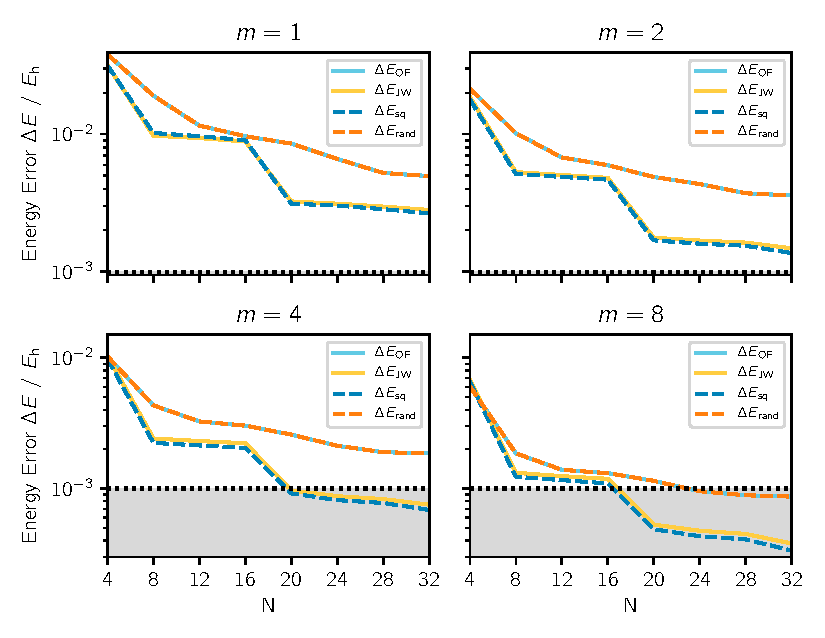
\includegraphics[width=4.5in]{figs/h6_error-N_order.pdf}
  \caption{Energy error $\Delta E$ (in $E_\mathrm{h}$) as a function of the number of Krylov basis states $N$ of \textbf{linear \ce{H6}} at a bond distance of 1.5~\AA.
   }
\label{h6_error-N}
\end{figure}
%%%%%%%%%%%%%%%%

Next, we examine how the effect of ordering might be change with different bond distances. Figure \ref{h6_pes} and Figure \ref{beh2_pes} show the potential energy curves (PEC) for \ce{H6} and \ce{BeH2}. For \methodabbr results, only \textbf{sq} and \textbf{rand} energies are plotted because they already well represent two asymptotic patterns.

We find that for \ce{H6} chain, the optimality of \textbf{sq} is consistent throughout the entire PEC (bond length from 0.6~\AA{}  to 2.0~\AA), which can be seen that the \textbf{sq} curves are always below the \textbf{rand} curves for these small Trotter number $m=1, 2, 4, 8$.
%%%%%% PES-H6 %%%%%%
\begin{figure}[h!]
  \centering
  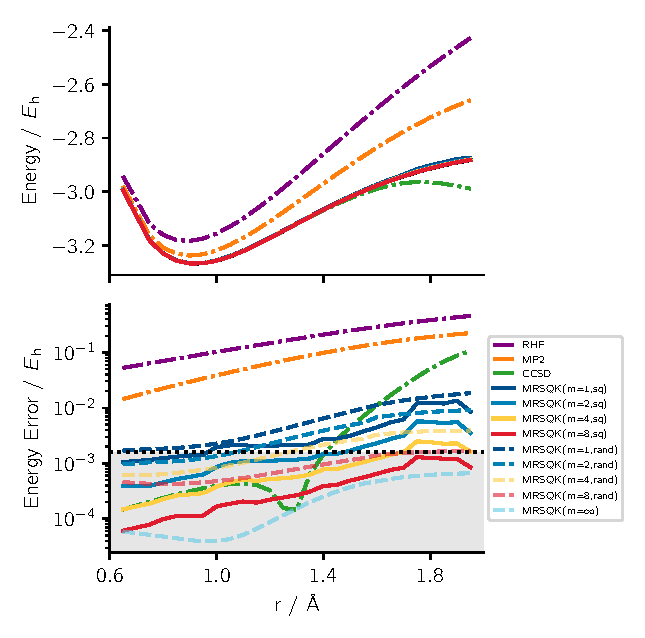
\includegraphics[width=3.2in]{figs/H6_pes_error.pdf}
  \caption{Potential energy curve (top) and energy error (bottom) for symmetric dissociation of \textbf{linear \ce{H6}} in STO-6G basis.
  References in \methodabbr were selected using initial QK calculations with $s_0 = 4$ evolutions of the Hartree-Fock determinant and a time step of $ \Delta t_0 = 0.25$ a.u.
  Then the following \methodabbr calculations use $ \Delta t = 0.5$ a.u., three time steps ($s=3$), and five references ($d=5$) corresponding to 20 Krylov basis states. 
  Two orderings of Pauli terms are employed for comparison, with notations consistent with that in Table~\ref{h6_gse_table}.
  The number of Trotter steps ($m$) is indicated in parentheses, while those from exact time evolution are labeled ($m = \infty$).
   }
\label{h6_pes}
\end{figure}
%%%%%%%%%%%%%%%%%

%%%%%% PEC-BeH2 %%%%%%
\begin{figure}[h!]
  \centering
  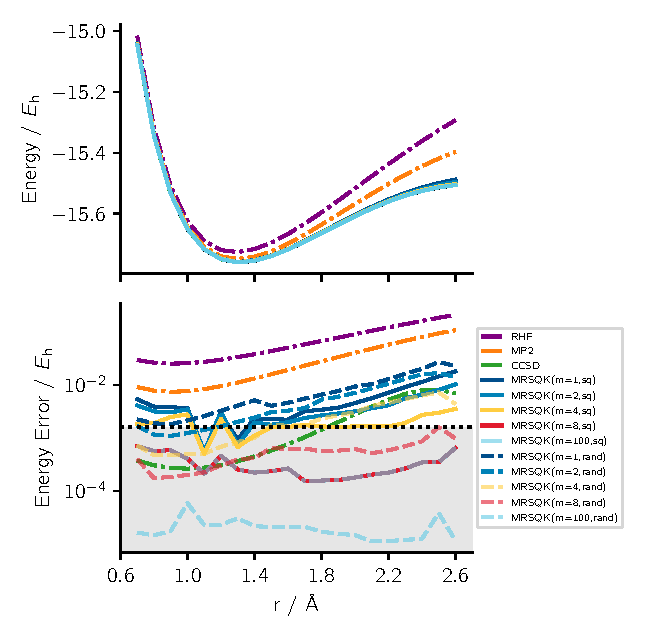
\includegraphics[width=3.2in]{figs/BeH2_pes_error.pdf}
  \caption{Potential energy curve (top) and energy error (bottom) for symmetric dissociation of \textbf{linear \ce{BeH2}} in STO-6G basis.
  References in \methodabbr were selected using initial QK calculations with $s_0 = 3$ evolutions of the Hartree-Fock determinant and a time step of $ \Delta t_0 = 0.25$ a.u.
  Then the following \methodabbr calculations use $ \Delta t = 2.0$ a.u., three time steps ($s=4$), and five references ($d=6$) corresponding to 30 Krylov basis states. 
  Two orderings of Pauli terms are employed for comparison, with notations consistent with that in Table~\ref{h6_gse_table}.
  The number of Trotter steps ($m$) is indicated in parentheses.
   }
\label{beh2_pes}
\end{figure}
%%%%%%%%%%%%%%%%%%%%%%%%%%%%%%%%%%%%
By scrutinizing the error plot, we observe some small discontinuities in the \textbf{sq} curves but none in the \textbf{rand} curves, which results from the fact that the optimal Trotter ordering varies with the bond length.\cite{tranter2019ordering}

The ordering effect in the PEC of \ce{BeH2} is much involved. In this case, the optimal ordering is not consistent when varying bond distances.
Most of the case \textbf{rand} ordering performs better, in both the energy error and the discontinuity problem. The \textbf{sq} ordering also suffer from the problem of slow convergence of energy with respect to the Trotter number $m$. We run the PEC calculations using a very large $m$ of 100, and surprisingly find that for \textbf{sq} ordering, the $m=100$ plot overlaps with $m=8$ plot entirely. This numerical observation is not well understood, thus requires further interrogation, which remains for future work.
%%%%%%%%%%%%%%%%%%%%%%%%%%%%%%%%%%%%
%%%%%%%%%%%%%%%%%%%%%%%%%%%%%%%%%%%%
\section{Conclusion}


%\section{Future Work}




\newpage
\bibliographystyle{achemso}
\bibliography{bibs/jan31export.bib,bibs/extra.bib,bibs/qkdrefs.bib}{}

\end{document}

